\documentclass{beamer}
\usepackage[utf8]{inputenc}
\usepackage[T1]{fontenc}
\usepackage[english]{babel}
\usepackage{url}
\usepackage{listings}
\usepackage{adjustbox}
\usepackage{chronology}
% \usepackage{sfmath}
%\usepackage{lxfonts}
%\usepackage{mathdesign}
\usepackage{unicode-math}

% Graphics
\usepackage{graphicx}
%\usepackage{tikz}
%\usetikzlibrary{matrix, calc, arrows, snakes}

% Figures
\usepackage{caption}
\captionsetup{labelformat=empty,labelsep=none}

% Font
\usepackage{microtype}
\usepackage{fontspec,xunicode}
\usepackage[scaled]{beramono}
\newfontfamily\sbmyriad{Myriad Pro Semibold}
\setsansfont{Myriad Pro}
\setbeamerfont{title}{family=\sbmyriad}
\setbeamerfont{frametitle}{family=\bf}

% Beamer theme settings
\usecolortheme{seagull}
\setbeamertemplate{itemize item}{\raisebox{0.8mm}{\rule{1.2mm}{1.2mm}}}
\usenavigationsymbolstemplate{} % no navigation buttons


\title{Master's thesis defence}
\subtitle{Option pricing with functional data-parallel languages}
\author{Philip Carlsen \and Martin Dybdal}
\date{22. March 2013}
\institute{Computer Science\\
University of Copenhagen}


\begin{document}
% Welcome
% Both a defence and this is what I do
\frame{\titlepage}

% % Nice diagram showing how the talk will progress
% \begin{frame}
%   \frametitle{Agenda}
%   \tableofcontents
% \end{frame}

\begin{frame}
  \frametitle{GPU Applications: Finance}
  \begin{figure}
    \centering
    Some cool finance graphics
    \caption{Option pricing}
\label{fig:gpufinance}
\end{figure}
\end{frame}
\begin{frame}
  \frametitle{GPU Applications: Bioinformatics}
  \begin{figure}
    \centering
    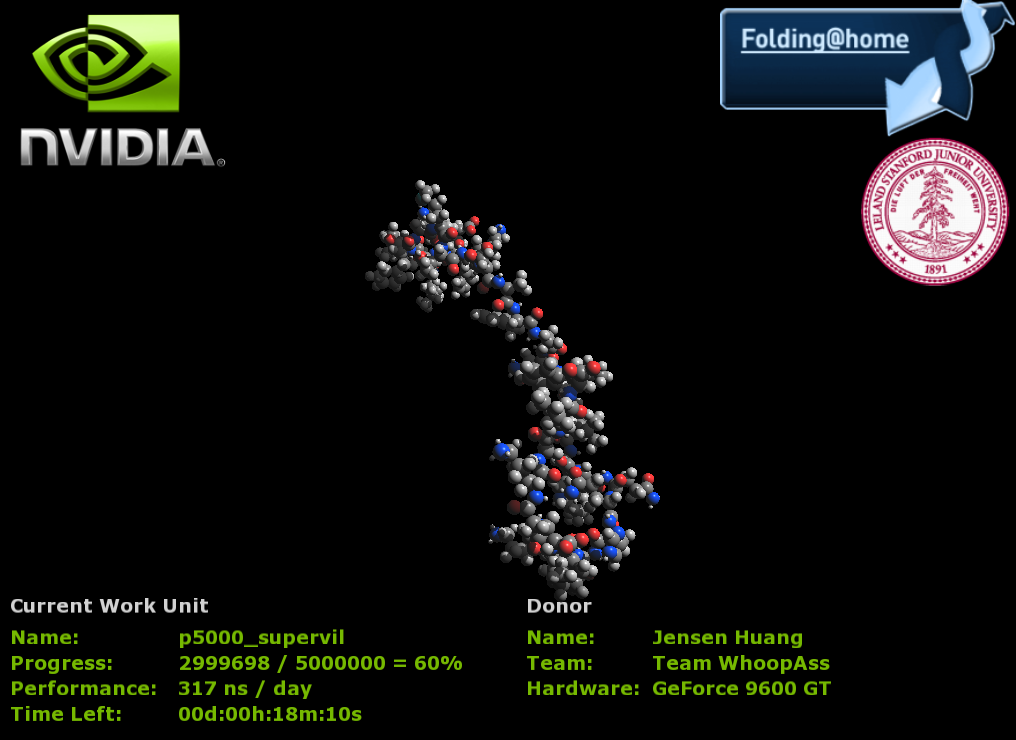
\includegraphics[width=0.8\textwidth]{graphics/fah_clientGeForce9600GT.png}
    \caption{Protein Folding}
\label{fig:foldingathome}
\end{figure}


  % \begin{itemize}
  % \item Computer vision
  % \item Scientific simulation (e.g. engineering, chemistry, physics)
  % \item Finance
  % \end{itemize}
\end{frame} 

\begin{frame}
  \frametitle{GPU Applications: Physics simulations}
  \begin{figure}
    \centering
    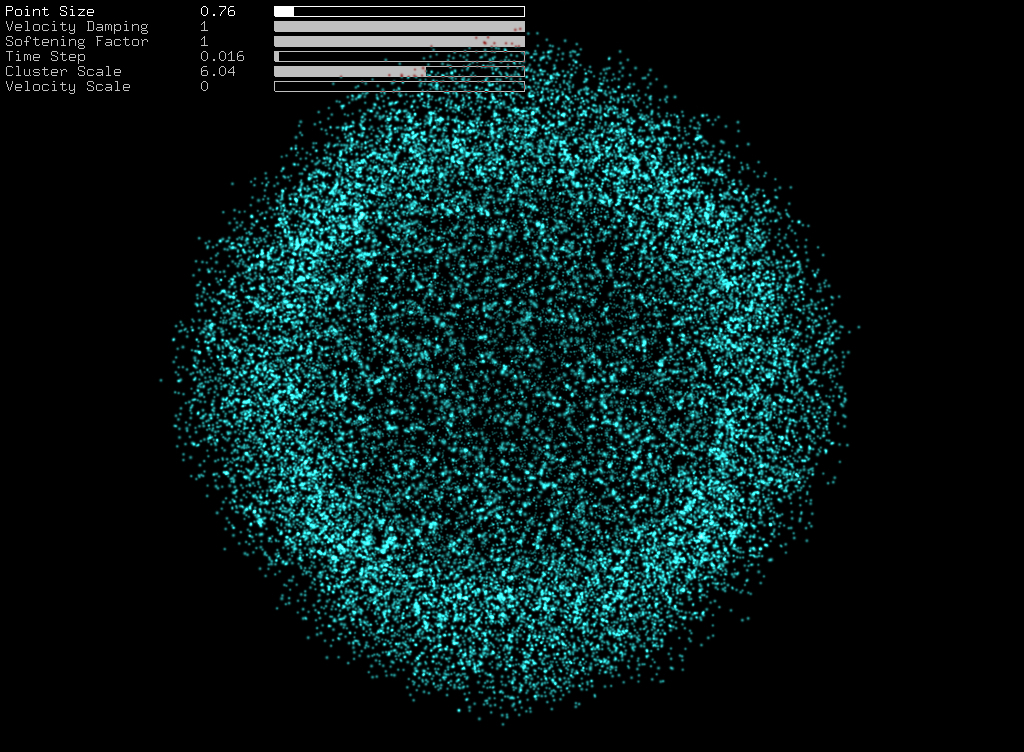
\includegraphics[width=0.8\textwidth]{graphics/opencl_nbody.jpg}
    \caption{N-body simulation}
\label{fig:simulation}
\end{figure}

\end{frame}
\begin{frame}
  \frametitle{GPU Applications: Medical imaging}

\end{frame}


\begin{frame}[t]
  \frametitle{GPUs vs. CPUs}
  \vspace{0.5cm}
   \begin{minipage}[t]{0.40\linewidth}
    NVIDIA GK104 GPU\\
    Multiprocessor\vspace{0.15cm}\\
    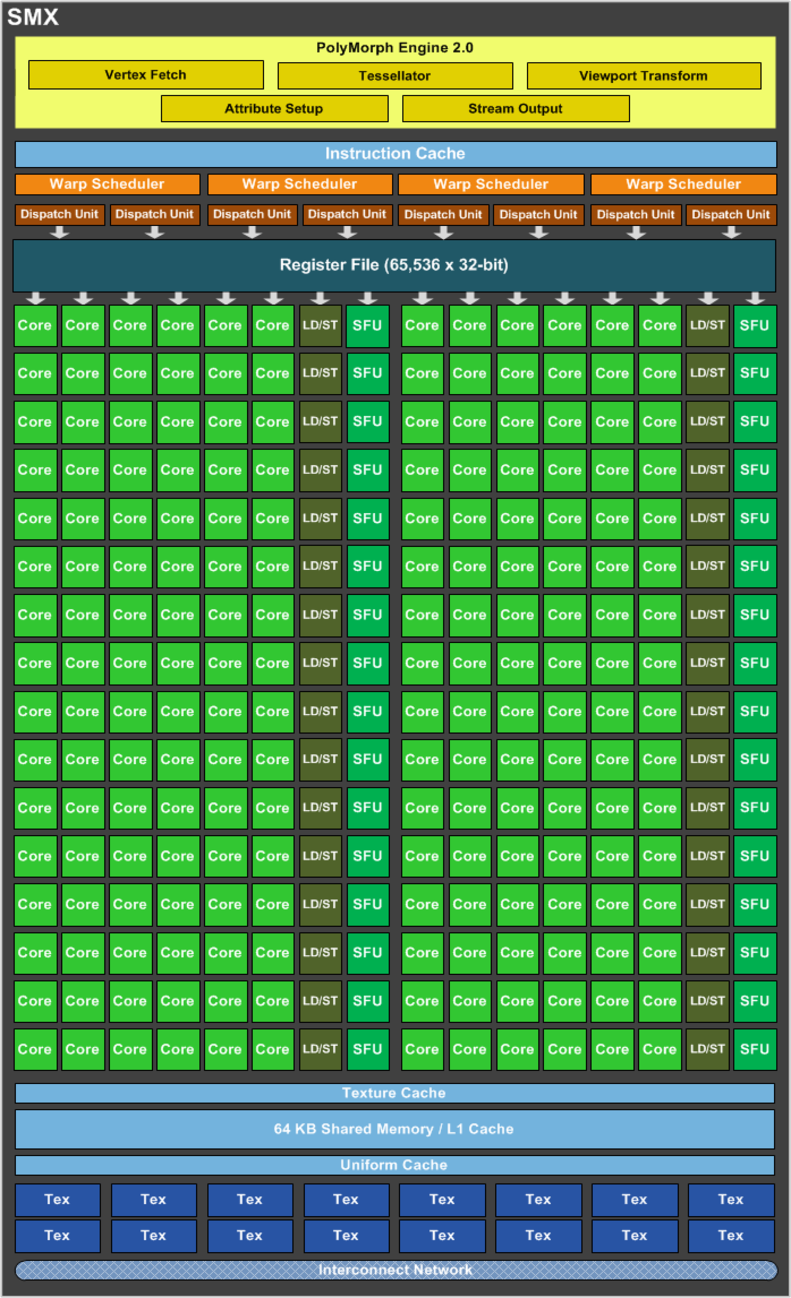
\includegraphics[width=0.8\textwidth]{graphics/nvidia_kepler_gk104_sm.pdf}
    % \begin{itemize}
    % \item 3540 mio. transistors
    % \item 1536 cores
    % \item Small caches
    % \item Many compute units
    % \item Optimized for throughput
    % \end{itemize}
  \end{minipage}
%  \pause
  \begin{minipage}[t]{0.55\linewidth}
    Intel Ivy Bridge CPU\vspace{0.15cm}\\
    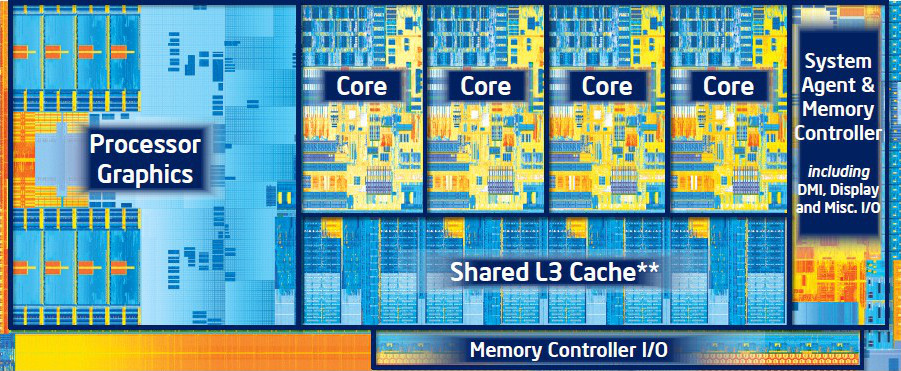
\includegraphics[width=\textwidth]{graphics/Intel-3rd-Generation-Ivy-Bridge-Processor.jpg}
    \begin{itemize}
    \item<1|only@1> Computation vs. Caching
    \item<1|only@1> SIMD vs. SISD
    \item<1|only@1> Throughput vs. latency
    \item<2-> Memory access coordination
    \item<3-> Avoid memory accesses\\ $\Rightarrow$ program fusion
    \item<4-> Schedule enough work
    \end{itemize}
  \end{minipage}
\end{frame}

% \begin{frame}
%   \frametitle{GPU programming concepts}
%   \begin{itemize}
%   \item Memory accesses are expensive
%   \item Coordination through memory coalescing
%   \item Compute on any single data item for as long as possible
%   \item Fusion
%   \item (Synchronization)
%   \item (SMs and blocks)
%   \end{itemize}
% \end{frame}

\begin{frame}
  \frametitle{GPU programming languages}

What we want:
  \begin{itemize}
  \item Avoid manual memory management
  \item Avoid manual fusion
  \item Fusion with library code
  \item Good abstractions
  \item Hardware independent
  \end{itemize}
\end{frame}

\begin{frame}
  \frametitle{Option styles}
\begin{adjustbox}{minipage=0.9\textwidth,center}
    \vspace{-4mm}
    \begin{chronology}[5]{2013}{2040}{3ex}{\textwidth}
      \event{2013}{now} \event{\decimaldate{1}{1}{2040}}{expiry}
    \end{chronology}\\
    European option

    \pause \vspace{7mm}
    \begin{chronology}[5]{2013}{2040}{3ex}{\textwidth}
      \event{2013}{now}
      \event[2020]{\decimaldate{1}{1}{2040}}{exercise time}
      \event{\decimaldate{1}{1}{2040}}{expiry}
    \end{chronology}
    American option

    \pause \vspace{7mm}
    \begin{chronology}[5]{2013}{2040}{3ex}{\textwidth}
      \event{2013}{now} \event{\decimaldate{1}{1}{2020}}{exercise
        time} \event{\decimaldate{1}{1}{2025}}{exercise time}
      \event{\decimaldate{1}{1}{2030}}{exercise time}
      \event{\decimaldate{1}{1}{2035}}{exercise time}
      \event{\decimaldate{1}{1}{2040}}{expiry}
    \end{chronology}
    Bermudan option
\end{adjustbox}

\end{frame}

% \fbox{  \begin{tikzpicture}
%     \node [] (now) at (0,0) {\rotatebox{-45}{\emph{now}}};
%     \node (expiry) at (8,0) {\rotatebox{-45}{\emph{expiry}}};
%     \draw[->,gray] (now) edge (expiry);

%     %\draw[->,gray,rounded corners] node[text=black,pos=.7]
% %    (now) -- (expiry);
%   \end{tikzpicture}
% }


% \begin{tikzpicture}[snake=zigzag, line before snake = 5mm, line after snake = 5mm]
% %draw horizontal line   
% \draw (0,0) -- (2,0);
% \draw[snake] (2,0) -- (4,0);
% \draw (4,0) -- (5,0);
% \draw[snake] (5,0) -- (7,0);

% %draw vertical lines
% \foreach \x in {0,1,2,4,5,7}
%    \draw (\x cm,3pt) -- (\x cm,-3pt);

% %draw nodes
% \draw (0,0) node[below=3pt] {$ 0 $} node[above=3pt] {$   $};
% \draw (1,0) node[below=3pt] {$ 1 $} node[above=3pt] {$ 10 $};
% \draw (2,0) node[below=3pt] {$ 2 $} node[above=3pt] {$ 20 $};
% \draw (3,0) node[below=3pt] {$  $} node[above=3pt] {$  $};
% \draw (4,0) node[below=3pt] {$ 5 $} node[above=3pt] {$ 50 $};
% \draw (5,0) node[below=3pt] {$ 6 $} node[above=3pt] {$ 60 $};
% \draw (6,0) node[below=3pt] {$  $} node[above=3pt] {$  $};
% \draw (7,0) node[below=3pt] {$ n $} node[above=3pt] {$ 10n $};
% \end{tikzpicture}

  % \begin{itemize}
  % \item Define american options
  % \item Binomial pricing
  % \item LSM
  % \item Sobol-sequence for sampling LSM paths
  % \end{itemize}


\begin{frame}
  \frametitle{Option pricing: Binomial method}
$$S(t+\Delta t) = \left\{
  \begin{array}{ll}
    S(t)u & \quad \text{with probability $q$} \\
    S(t)d & \quad \text{with probability $1-q$}
  \end{array} \right.
$$

\begin{figure}
  \centering
  \tikzstyle{nodestyle} = [text centered, minimum size=0.42cm, inner sep=0]

\begin{tikzpicture}
  \node at (0,0) [nodestyle] (S1) {$S(t_0)$};

  \node at (-1, -1) [nodestyle] (dS) {$dS(t_0)$};
  \node at ( 1, -1) [nodestyle] (uS) {$uS(t_0)$};

  \node at ( 2, -2) [nodestyle] (u2S) {$u^2S(t_0)$};
  \node at ( 0, -2) [nodestyle] (S2) {$S(t_0)$};
  \node at (-2, -2) [nodestyle] (d2S) {$d^2S(t_0)$};

  \node at ( 3, -3) [nodestyle] (u3S) {$u^3S(t_0)$};
  \node at ( 1, -3) [nodestyle] (uS2) {$uS(t_0)$};
  \node at (-1, -3) [nodestyle] (dS2) {$dS(t_0)$};
  \node at (-3, -3) [nodestyle] (d3S) {$d^3S(t_0)$};

  \node at (-4.5,  0) [] (t0) {$S(t_0) =$};
  \node at (-4.5, -1) [] (t0) {$S(t_1) =$};
  \node at (-4.5, -2) [] (t0) {$S(t_2) =$};
  \node at (-4.5, -3) [] (t0) {$S(t_3) =$};

  \path[-latex]
     (S1) edge (uS)
     (S1) edge (dS)

     (uS) edge (S2)
     (dS) edge (S2)
     (uS) edge (u2S)
     (dS) edge (d2S)

     (u2S) edge (u3S)
     (u2S) edge (uS2)
     (S2)  edge (uS2)
     (S2)  edge (dS2)
     (d2S) edge (dS2)
     (d2S) edge (d3S);
\end{tikzpicture}

\vspace{2mm}

\caption{Binomial lattice for three periods ($u\cdot d = 1$)}
\label{fig:binomial-tree}
\end{figure}
  
\end{frame}

\begin{frame}
  \frametitle{Option pricing: Least-Squares Monte Carlo}
  
\end{frame}

\begin{frame}
  \frametitle{Sobol sequences generation}
  
\end{frame}

\begin{frame}
  \frametitle{The case for nested array operations}
  Present example of a program that gets incomprehensible and
  incomposable in Nikola and Accelerate.
\end{frame}

\begin{frame}[fragile]
  \frametitle{Solution \#1: Accelerate-style}
  \begin{itemize}
  \item We are lucky, that in our case an alternative (an even a
    more efficient) algorithm
    exists
  \item Accelerate-style ``add a dimension'' unfold
  \end{itemize}

{\footnotesize
\begin{verbatim}
unfold :: (Shape sh, Elem a)
       => Int -> (Int -> a -> a)
       -> Array sh a -> Array (sh :. Int) a
\end{verbatim} }

% {\footnotesize
% \begin{verbatim}
% unfold :: (IsElem a, IsElem (Exp t Ix), Shape sh, Source r a)
%        => Exp t Ix
%        -> (Exp t Ix -> a -> a)
%        -> Array r sh a
%        -> Array PSH (sh :. Exp t Ix) a
% \end{verbatim} }
\end{frame}

\begin{frame}
  \frametitle{How it breaks down}
  \begin{itemize}
  \item Composability is lost.
  \item Will it still break down if we wrap it in another map?
  \end{itemize}
\end{frame}

\begin{frame}
  \frametitle{Solution \#2: Nested array operations}
  \begin{itemize}
  \item mapNest and unfold
  \item Now we have another problem! Where is the parallelism going in (map (foldl (map ..) ..) ..)
  \end{itemize}
\end{frame}

\begin{frame}
  \frametitle{Solution \#2: Sequential}
  \begin{itemize}
  \item Present informal semantics
  \item We are far from finished implementing it in Nikola
  \item We used the last two weeks implementing a quick demo
  \end{itemize}
\end{frame}

\begin{frame}
  \frametitle{Solution \#3: Sequential}
  \begin{itemize}
  \item Demo introduction
  \end{itemize}
\end{frame}

\begin{frame}
  \frametitle{Solution \#2: Sequential}
  \begin{itemize}
  \item Fusion
  \end{itemize}
\end{frame}

\begin{frame}
  \frametitle{Future work}
\end{frame}

\end{document}

%%% Local Variables:
%%% mode: latex
%%% TeX-engine: luatex
%%% End: